% Options for packages loaded elsewhere
% Options for packages loaded elsewhere
\PassOptionsToPackage{unicode}{hyperref}
\PassOptionsToPackage{hyphens}{url}
%
\documentclass[
  ignorenonframetext,
  aspectratio=169,
  handout]{beamer}
\newif\ifbibliography
\usepackage{pgfpages}
\setbeamertemplate{caption}[numbered]
\setbeamertemplate{caption label separator}{: }
\setbeamercolor{caption name}{fg=normal text.fg}
\beamertemplatenavigationsymbolsempty
% remove section numbering
\setbeamertemplate{part page}{
  \centering
  \begin{beamercolorbox}[sep=16pt,center]{part title}
    \usebeamerfont{part title}\insertpart\par
  \end{beamercolorbox}
}
\setbeamertemplate{section page}{
  \centering
  \begin{beamercolorbox}[sep=12pt,center]{section title}
    \usebeamerfont{section title}\insertsection\par
  \end{beamercolorbox}
}
\setbeamertemplate{subsection page}{
  \centering
  \begin{beamercolorbox}[sep=8pt,center]{subsection title}
    \usebeamerfont{subsection title}\insertsubsection\par
  \end{beamercolorbox}
}
% Prevent slide breaks in the middle of a paragraph
\widowpenalties 1 10000
\raggedbottom
\AtBeginPart{
  \frame{\partpage}
}
\AtBeginSection{
  \ifbibliography
  \else
    \frame{\sectionpage}
  \fi
}
\AtBeginSubsection{
  \frame{\subsectionpage}
}
\usepackage{iftex}
\ifPDFTeX
  \usepackage[T1]{fontenc}
  \usepackage[utf8]{inputenc}
  \usepackage{textcomp} % provide euro and other symbols
\else % if luatex or xetex
  \usepackage{unicode-math} % this also loads fontspec
  \defaultfontfeatures{Scale=MatchLowercase}
  \defaultfontfeatures[\rmfamily]{Ligatures=TeX,Scale=1}
\fi
\usepackage{lmodern}

\ifPDFTeX\else
  % xetex/luatex font selection
\fi
% Use upquote if available, for straight quotes in verbatim environments
\IfFileExists{upquote.sty}{\usepackage{upquote}}{}
\IfFileExists{microtype.sty}{% use microtype if available
  \usepackage[]{microtype}
  \UseMicrotypeSet[protrusion]{basicmath} % disable protrusion for tt fonts
}{}
\makeatletter
\@ifundefined{KOMAClassName}{% if non-KOMA class
  \IfFileExists{parskip.sty}{%
    \usepackage{parskip}
  }{% else
    \setlength{\parindent}{0pt}
    \setlength{\parskip}{6pt plus 2pt minus 1pt}}
}{% if KOMA class
  \KOMAoptions{parskip=half}}
\makeatother


\usepackage{longtable,booktabs,array}
\newcounter{none} % for unnumbered tables
\usepackage{calc} % for calculating minipage widths
\usepackage{caption}
% Make caption package work with longtable
\makeatletter
\def\fnum@table{\tablename~\thetable}
\makeatother
\usepackage{graphicx}
\makeatletter
\newsavebox\pandoc@box
\newcommand*\pandocbounded[1]{% scales image to fit in text height/width
  \sbox\pandoc@box{#1}%
  \Gscale@div\@tempa{\textheight}{\dimexpr\ht\pandoc@box+\dp\pandoc@box\relax}%
  \Gscale@div\@tempb{\linewidth}{\wd\pandoc@box}%
  \ifdim\@tempb\p@<\@tempa\p@\let\@tempa\@tempb\fi% select the smaller of both
  \ifdim\@tempa\p@<\p@\scalebox{\@tempa}{\usebox\pandoc@box}%
  \else\usebox{\pandoc@box}%
  \fi%
}
% Set default figure placement to htbp
\def\fps@figure{htbp}
\makeatother





\setlength{\emergencystretch}{3em} % prevent overfull lines

\providecommand{\tightlist}{%
  \setlength{\itemsep}{0pt}\setlength{\parskip}{0pt}}



 


\makeatletter
\@ifpackageloaded{caption}{}{\usepackage{caption}}
\AtBeginDocument{%
\ifdefined\contentsname
  \renewcommand*\contentsname{Table of contents}
\else
  \newcommand\contentsname{Table of contents}
\fi
\ifdefined\listfigurename
  \renewcommand*\listfigurename{List of Figures}
\else
  \newcommand\listfigurename{List of Figures}
\fi
\ifdefined\listtablename
  \renewcommand*\listtablename{List of Tables}
\else
  \newcommand\listtablename{List of Tables}
\fi
\ifdefined\figurename
  \renewcommand*\figurename{Figure}
\else
  \newcommand\figurename{Figure}
\fi
\ifdefined\tablename
  \renewcommand*\tablename{Table}
\else
  \newcommand\tablename{Table}
\fi
}
\@ifpackageloaded{float}{}{\usepackage{float}}
\floatstyle{ruled}
\@ifundefined{c@chapter}{\newfloat{codelisting}{h}{lop}}{\newfloat{codelisting}{h}{lop}[chapter]}
\floatname{codelisting}{Listing}
\newcommand*\listoflistings{\listof{codelisting}{List of Listings}}
\makeatother
\makeatletter
\makeatother
\makeatletter
\@ifpackageloaded{caption}{}{\usepackage{caption}}
\@ifpackageloaded{subcaption}{}{\usepackage{subcaption}}
\makeatother

\usepackage{bookmark}
\IfFileExists{xurl.sty}{\usepackage{xurl}}{} % add URL line breaks if available
\urlstyle{same}
\hypersetup{
  pdftitle={The Classical Harmonic Oscillator},
  pdfauthor={Davit Potoyan},
  hidelinks,
  pdfcreator={LaTeX via pandoc}}


\title{\texorpdfstring{The Classical Harmonic
Oscillator}{The Classical Harmonic Oscillator}}
\subtitle{\texorpdfstring{Chem 3240 · Lecture
4.2}{Chem 3240 · Lecture 4.2}}
\author{Davit Potoyan}
\date{}

\begin{document}
\frame{\titlepage}


\begin{frame}
\begin{block}{Bead, spring, and a wall}
\protect\phantomsection\label{bead-spring-and-a-wall}
\begin{columns}[T]
\begin{column}{0.55\linewidth}
\begin{itemize}
\tightlist
\item
  A mass tied to a wall by a spring
\item
  Displace it by \(x\) from equilibrium
\item
  A \textbf{restoring force} pulls it back
\end{itemize}

\[F = -kx\]

The minus sign always points \textbf{toward equilibrium}
\end{column}

\begin{column}{0.45\linewidth}
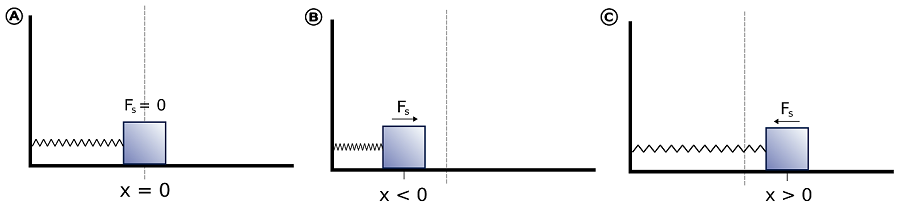
\includegraphics[width=1\linewidth,height=\textheight,keepaspectratio]{../../ch04/images/harm-osc1.png}
\end{column}
\end{columns}
\end{block}

\begin{block}{Hooke's law}
\protect\phantomsection\label{hookes-law}
\[F = -kx\]

\begin{itemize}
\tightlist
\item
  \(k\) is the \textbf{spring constant}: the stiffness
\item
  Stiffer spring means a stronger pull back
\item
  The only ingredient we need to build the whole model
\end{itemize}
\end{block}

\begin{block}{Equation of motion}
\protect\phantomsection\label{equation-of-motion}
\begin{itemize}
\tightlist
\item
  Newton's second law with the Hooke force:
\end{itemize}

\[m\ddot{x} = -kx\]

\[\ddot{x} + \omega^2 x = 0\]

\begin{itemize}
\tightlist
\item
  A linear \textbf{second-order ODE}
\item
  One constant \(\omega\) governs everything
\end{itemize}
\end{block}

\begin{block}{The solution}
\protect\phantomsection\label{the-solution}
\begin{columns}[T]
\begin{column}{0.55\linewidth}
\[x(t) = A\cos(\omega t + \phi)\]

\begin{itemize}
\tightlist
\item
  \textbf{Amplitude} \(A\) and \textbf{phase} \(\phi\) set by initial
  conditions
\item
  Motion is a pure cosine: \textbf{simple harmonic motion}
\end{itemize}
\end{column}

\begin{column}{0.45\linewidth}
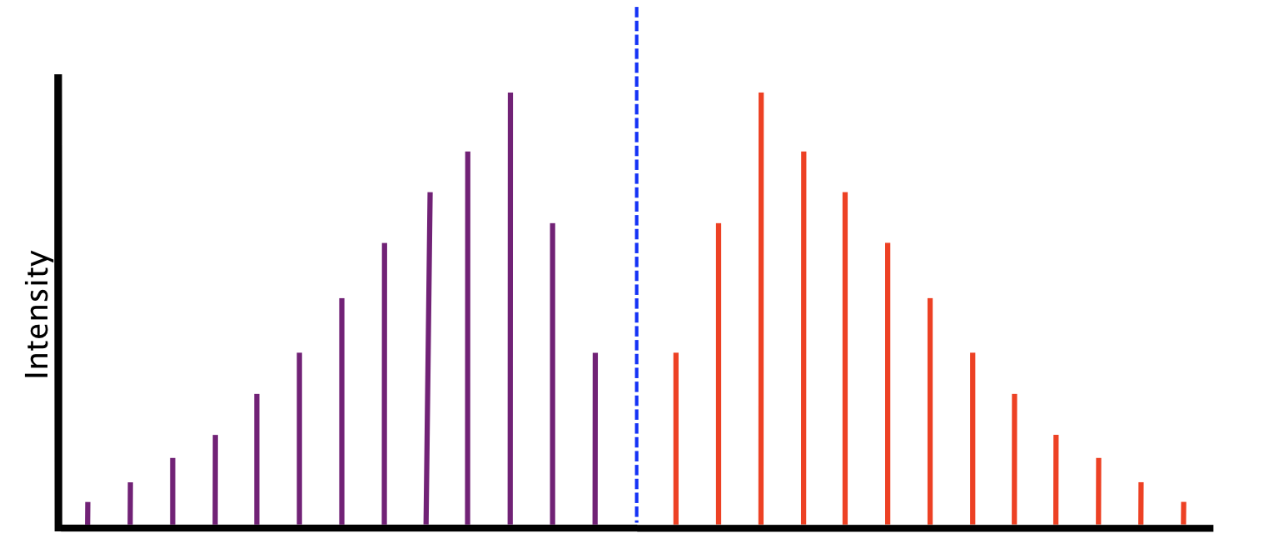
\includegraphics[width=1\linewidth,height=\textheight,keepaspectratio]{../../ch04/images/ideal.png}
\end{column}
\end{columns}
\end{block}

\begin{block}{Frequency}
\protect\phantomsection\label{frequency}
\[\omega = \sqrt{\frac{k}{\mu}}\]

\begin{itemize}
\tightlist
\item
  \textbf{Stiffer} spring (larger \(k\)): faster oscillation
\item
  \textbf{Heavier} mass (larger \(\mu\)): slower oscillation
\item
  Period \(T = 2\pi/\omega\), frequency \(f = \omega/2\pi\)
\end{itemize}
\end{block}

\begin{block}{Energy of the oscillator}
\protect\phantomsection\label{energy-of-the-oscillator}
\begin{columns}[T]
\begin{column}{0.55\linewidth}
\begin{itemize}
\tightlist
\item
  Force is the slope of a potential: \(F = -\partial V/\partial x\)
\item
  Integrating gives a \textbf{parabolic well}: \(V = \tfrac{1}{2}kx^2\)
\end{itemize}

\[E = \frac{p^2}{2m} + \frac{kx^2}{2}\]

\begin{itemize}
\tightlist
\item
  Kinetic and potential energy trade off; \textbf{total energy is
  constant}
\end{itemize}
\end{column}

\begin{column}{0.45\linewidth}
\includegraphics[width=1\linewidth,height=\textheight,keepaspectratio]{../../ch04/images/ext_shm_graphs.gif}
\end{column}
\end{columns}
\end{block}

\begin{block}{Diatomic molecule: a two-body problem}
\protect\phantomsection\label{diatomic-molecule-a-two-body-problem}
\begin{itemize}
\tightlist
\item
  Two atoms bound by a spring, masses \(m_1\) and \(m_2\)
\item
  Center of mass drifts freely; only the \textbf{relative coordinate}
  vibrates
\end{itemize}

\[\ddot{x} = -\left(\frac{1}{m_1} + \frac{1}{m_2}\right)kx = -\frac{k}{\mu}x\]
\end{block}

\begin{block}{Reduced mass}
\protect\phantomsection\label{reduced-mass}
\begin{itemize}
\tightlist
\item
  The two-body problem becomes \textbf{one body} with an effective mass:
\end{itemize}

\[\mu = \frac{m_1 m_2}{m_1 + m_2}\]

\begin{itemize}
\tightlist
\item
  Same equation as the bead on a wall, with \(m \to \mu\)
\item
  One particle, one spring, one frequency \(\omega = \sqrt{k/\mu}\)
\end{itemize}
\end{block}

\begin{block}{Real bonds are not parabolas}
\protect\phantomsection\label{real-bonds-are-not-parabolas}
\begin{columns}[T]
\begin{column}{0.5\linewidth}
\begin{itemize}
\tightlist
\item
  Real bonds \textbf{dissociate}; a parabola never does
\item
  Taylor expand any well about its minimum \(x_0\):
\end{itemize}
\end{column}

\begin{column}{0.5\linewidth}
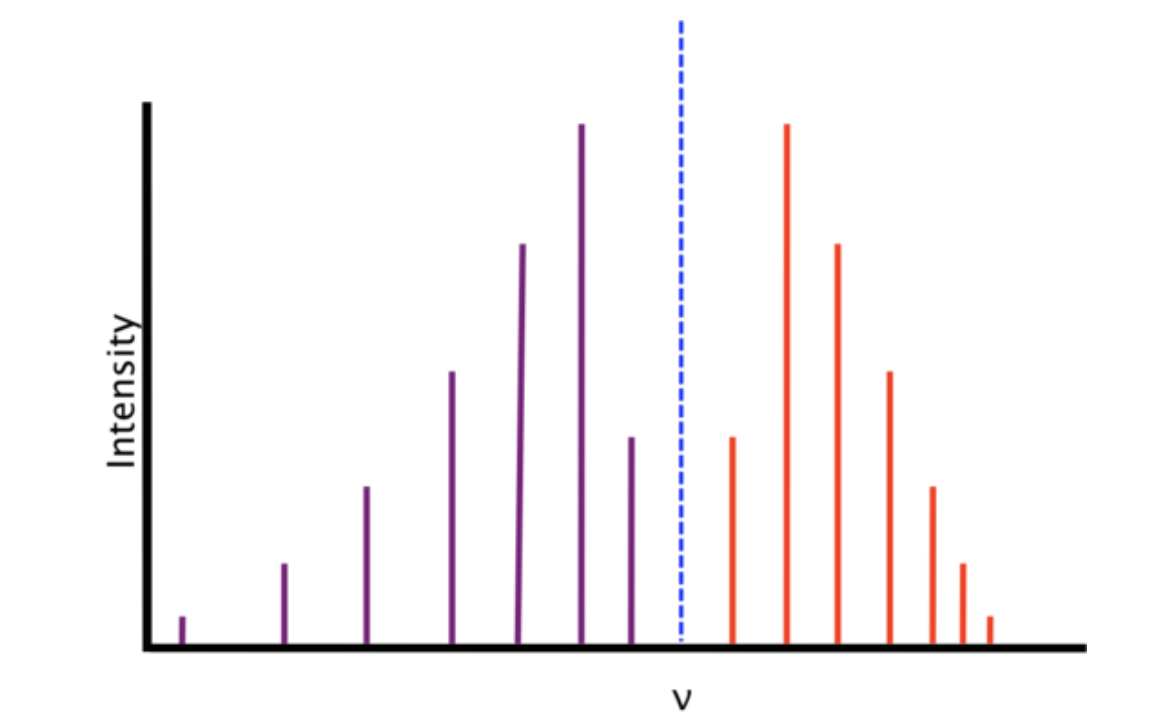
\includegraphics[width=1\linewidth,height=\textheight,keepaspectratio]{../../ch04/images/real.png}
\end{column}
\end{columns}

\[U(x) = \frac{1}{2}k(x-x_0)^2 + \frac{1}{6}\gamma(x-x_0)^3 + \cdots\]
\end{block}

\begin{block}{The harmonic approximation}
\protect\phantomsection\label{the-harmonic-approximation}
\begin{columns}[T]
\begin{column}{0.55\linewidth}
\begin{itemize}
\tightlist
\item
  First derivative vanishes at the minimum
\item
  Keep only the \textbf{first non-vanishing term}: the quadratic
\item
  \(k\) is the \textbf{curvature} \(U''(x_0)\) at the bottom of the well
\item
  Good near equilibrium; \textbf{anharmonic} terms grow far out
\end{itemize}
\end{column}

\begin{column}{0.45\linewidth}
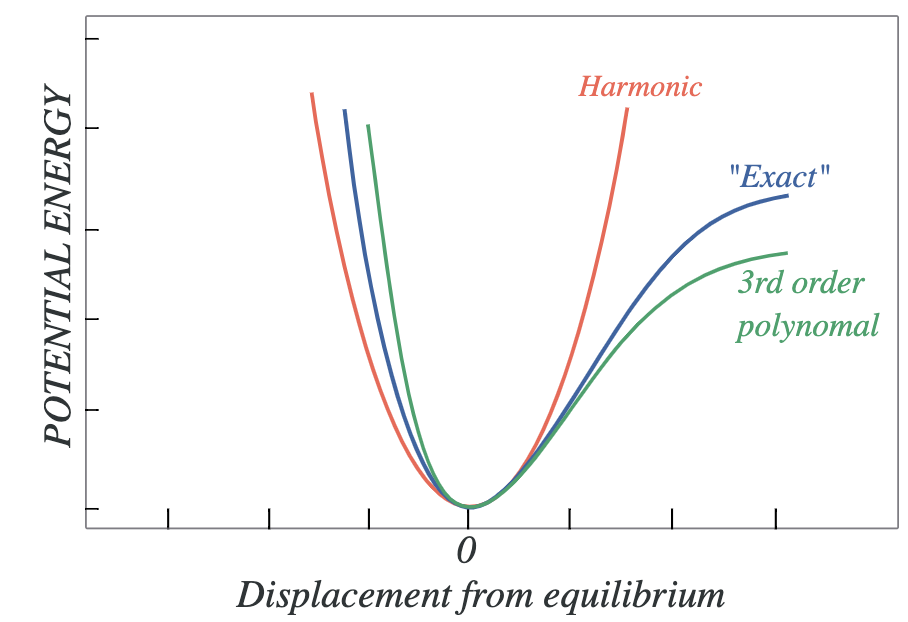
\includegraphics[width=1\linewidth,height=\textheight,keepaspectratio]{../../ch04/images/harm_approx.png}
\end{column}
\end{columns}
\end{block}
\end{frame}

\begin{frame}{Takeaway}
\protect\phantomsection\label{takeaway}
\begin{quote}
A restoring force \(F=-kx\) gives sinusoidal motion
\(x(t)=A\cos(\omega t+\phi)\) at \(\omega=\sqrt{k/\mu}\). Any bond near
its minimum is harmonic, and the parabola is the launching point for the
quantum oscillator.
\end{quote}
\end{frame}




\end{document}
